\documentclass[10pt]{article}

\IfFileExists{colm2026_conference.sty}{%
  \usepackage{colm2026_conference}
}{%
  \usepackage[margin=0.85in]{geometry}
}

\usepackage[T1]{fontenc}
\usepackage[utf8]{inputenc}
\usepackage{times}
\usepackage{microtype}
\usepackage{amsmath,amssymb}
\usepackage{booktabs}
\usepackage{tabularx}
\usepackage{array}
\usepackage{xcolor}
\usepackage{tikz}
\usepackage{placeins}
\usepackage{hyperref}
\usepackage[numbers,sort&compress]{natbib}

\usetikzlibrary{arrows.meta,positioning,fit,backgrounds}

\hypersetup{
  colorlinks=true,
  linkcolor=blue!45!black,
  citecolor=blue!45!black,
  urlcolor=blue!45!black
}

\newcolumntype{Y}{>{\raggedright\arraybackslash}X}
\newcommand{\method}{Gauss6/\allowbreak FullVA}
\newcommand{\fullva}{FullVA}
\newcommand{\tfe}{TFE}
\newcommand{\status}[1]{\texttt{#1}}

\tikzset{
  box/.style={draw=blue!55!black, fill=blue!5, rounded corners=2pt,
    align=center, inner sep=4pt, font=\small},
  vbox/.style={draw=green!45!black, fill=green!7, rounded corners=2pt,
    align=center, inner sep=4pt, font=\small},
  warn/.style={draw=orange!75!black, fill=orange!8, rounded corners=2pt,
    align=center, inner sep=4pt, font=\small},
  stop/.style={draw=red!65!black, fill=red!7, rounded corners=2pt,
    align=center, inner sep=4pt, font=\small},
  arr/.style={-{Latex[length=2mm]}, thick, draw=black!65}
}

\title{A Verifier-Centered Method for Discovering New Integrators:\\
A 48-Version LLM-Assisted Case Study}

\author{Anonymous Authors}
\date{}

\begin{document}
\maketitle

\begin{abstract}
We describe a verifier-centered method for using LLM agents to discover new
scientific-computing integrators. The method is studied through an anonymized
48-version search in Lie-group constrained multibody integration, a deliberately
hard setting where a useful integrator must preserve manifold kinematics, solve
index-3 constrained dynamics, represent lower-pair multipliers and friction,
and keep residual rows, endpoint repairs, and comparison policies from
silently changing the one-step map being tested. The paper's primary subject is
the discovery method, not the integrator formula alone: inherited
Lie-kinematic, Gauss, ASME-mechanism, \tfe{}/Lobatto, friction, and
external-harness directions are stored as verifier questions rather than
leaderboard rows. The agent maintains MethodSpec, ProblemSpec, EvidenceSpec,
ClaimSpec, and ledger objects, turning four ASME mechanisms into a
verifier-controlled test environment: single and double pendulum carry
dynamic-order gates, while four-link and slider-crank carry closed-loop
coverage and reaction-consistency gates. Across the ledger, failed
endpoint-constrained DAE solves, direct Lobatto swaps, projection repairs, and
sparse-Jacobian speed paths become next-version constraints. The discovered
discovered outcome is a bounded sixth-order \method{} claim, with smooth observed
position/velocity orders 7.161/7.066 and a 132-row residual certificate
boundary; complete source-paper \tfe{} replacement, external superiority,
sparse runtime superiority, and dynamic order for the closed-loop rows remain
unpromoted. The contribution is the verifier-centered discovery procedure:
LLM agents become scientifically useful when they preserve the narrowing path
and claim boundary, not when they merely automate research prose or count
artifacts.
\end{abstract}

\section{Introduction}

Lie-group constrained multibody integration is difficult because the method is
defined by more than an update formula. The difficult part is not proposing
another quadrature rule; it is preserving the identity of the residual being
solved. Rotations live on a manifold, while the mechanical equations form a
constrained differential-algebraic system with position-, velocity-, and
acceleration-level consequences
\citep{Hairer1996SolvingII,MuntheKaas1998RK}. Lower-pair joints introduce
multipliers and reaction forces, friction makes smoothness regime-dependent,
and Newton residual rows decide which one-step map is actually being solved.
A clean convergence plot can therefore be misleading: it may hide endpoint
projection, a changed reference policy, a lower-dimensional surrogate, or a
diagnostic residual that is not the claimed method.

This setting is exactly where an agentic research system is tempting and
dangerous. A language model can inspect code, propose residual variants, run
sweeps, summarize failures, and maintain long experiment histories. But if the
agent also rewrites reports and proof notes, the key failure mode is claim
drift. A partial result can be described as a method, a mechanism-coverage row
can be described as dynamic order, or an external comparison scaffold can be
described as superiority. The scientific problem is therefore not just whether
an agent can run experiments. It is whether the agent can help discover a
method while preserving the exact boundary of what has been shown.

The project did not start from a clean leaderboard. It inherited Lie-group
kinematic baselines, reduced conservative mechanics, absolute-coordinate DAE
prototypes, frictional tests, temporal-finite-element targets, public-code ASME
mechanisms, and external comparison policies. We treated these objects as typed
verifier questions: each could explain part of the behavior, but none could by itself
define the final \method{} claim. This distinction matters because a local
reproduction, a reduced surrogate, a source-paper formula target, and a public
same-test row are different evidence objects.

The central design decision was to make those distinctions explicit in the
research environment. The state was represented as method, problem, evidence,
claim, and ledger objects. The agent could propose hypotheses and execute
bounded experiments, but it could not change a claim state until a
domain-specific validator checked method identity, problem specification,
evidence artifact, and wording boundary. The four ASME mechanisms were then
used as a test environment rather than a flat leaderboard: single and double
pendulum test local dynamic order, while four-link and slider-crank test
closed-loop lower-pair coverage and reaction consistency.

This conservative design was not imposed fully formed. It emerged through 48
versions as a five-block narrowing chain: representation and public-baseline
locks; constrained-DAE identity tests around endpoint policy, V/A level,
friction, and transport; Gauss6 retained while trapezoidal, BDF, Lobatto, and
reduced surrogates became verifier questions; endpoint-node and projection
explanations rejected in favor of stage-level lower-pair V/A rows; and later
sparse, closed-loop, source-policy, and external-comparison paths kept as claim
boundaries. The story is not that many versions were attempted, but that failed
explanations became next-version constraints until the surviving method
identity became \method{}.

Only after this numerical-method dependency chain is fixed do recent
LLM-for-science systems become relevant. LLMs have been used for scientific
literature synthesis, tool use, program search, chemical planning, autonomous
experimentation, and broader end-to-end research loops
\citep{Wang2023AIScience,Boiko2023Coscientist,
Bran2024ChemCrow,RomeraParedes2024FunSearch,Lu2024AIScientist}. LM4Sci 2026
explicitly calls for LLM agents that accelerate complex scientific workflows,
support human-AI collaboration, and evaluate AI-generated research artifacts
\citep{LM4Sci2026CFP}. We study a narrow version of that agenda: a single
scientific-computing case used to describe a verifier-centered method for
discovering new integrators with LLM agents.

The contribution is the discovery method and its auditable case study, not a
standalone paper whose main goal is to describe the \method{} integrator, not a
generic prompt recipe, and not a paper-writing pipeline. Paper drafting,
formatting, and review scaffolds are downstream packaging; they are not the
scientific object studied here. The object is the procedure that made the
\method{} method identifiable while keeping stronger claims out of the
accepted state.
We make three claims:

\begin{enumerate}
  \item A verifier-centered integrator-discovery method can make agentic search
  auditable by separating method, problem, evidence, claim, and ledger objects
  before claims are promoted.
  \item Inherited numerical methods, public mechanisms, failed variants, and
  external harnesses can be treated as typed verifier questions, so that each
  48-version transition records what was retained, rejected, or quarantined.
  \item In this case, the discovery method isolates a bounded \method{} outcome
  while preventing endpoint repair, sparse diagnostics, full \tfe{}
  replacement, and external-comparison scaffolds from becoming unsupported
  claims.
\end{enumerate}

\section{Related Work and Gap}

The prior work that mattered first was numerical. Classical DAE analysis and
Lie-group time stepping explain why residual identity, constraint level, and
manifold transport matter \citep{Hairer1996SolvingII,MuntheKaas1998RK}. The
local project also inherited practical baselines: right-action kinematics,
reduced conservative mechanics, ASME-style public mechanisms, trapezoidal/BDF
and Lobatto directions, a Gauss-Lobatto/\tfe{} source target, friction variants,
sparse/backend probes, and external same-test harnesses. These were not
after-the-fact citations; they initialized representation locks, local
baselines, rejected explanations, and comparison boundaries the final claim
could not exceed.
We therefore treat them as verifier questions, not a leaderboard: representation
trust, local validity, endpoint-map changes, and forbidden scaling/external
promotion. Table \ref{tab:comparators} summarizes their roles in the discovery
story.

\begin{table}[!htbp]
\centering
\caption{Inherited directions used as typed verifier questions in the discovery
process.}
\label{tab:comparators}
\small
\begin{tabularx}{\linewidth}{p{0.25\linewidth}YY}
\toprule
\textbf{Comparator family} & \textbf{Role in the search} & \textbf{Boundary} \\
\midrule
Lie-group kinematics and RKMK/CF updates & Fixed right-action rotation
conventions and high-order attitude transport. & Does not close constrained
DAE dynamics. \\
Conservative Lie midpoint/Gauss mechanics & Showed that smooth rigid-body
mechanics could be made high order. & Does not handle lower-pair
constraints, multipliers, and friction. \\
ASME-style public mechanisms & Supplied reproducibility anchors and
reviewer-facing examples. & A reproduction anchor is not a new \method{}
claim. \\
Trapezoidal, BDF, and Lobatto baselines & Tested lower-order, damping, and
endpoint-node explanations. & Reduced baselines do not prove the full
absolute-coordinate lower-pair method. \\
Gauss-Lobatto/\tfe{} target & Provided a stronger source-reproduction
direction and expected-order comparator. & Current accepted method does not
claim complete source-paper \tfe{} residual replacement. \\
Friction and multiplier-dependent load variants & Stressed smooth versus
sharp regimes and reaction-dependent forcing. & Smooth and sharp order
statements must remain separate. \\
Scaling and external-policy harnesses & Measured sparse/backend pressure from
larger FullVA systems and organized public-code/common-window rows. & Neither
backend correctness nor same-test scaffolding defines method order, sparse
speed, or external superiority. \\
\bottomrule
\end{tabularx}
\end{table}

The LLM-for-science context supplies a different motivation. Automation of
science predates modern LLMs \citep{King2009AutomationScience}, and recent
systems use foundation models as interfaces over literature, code, tools, and
workflow state: Coscientist and ChemCrow coordinate chemistry and laboratory
tasks \citep{Boiko2023Coscientist,Bran2024ChemCrow}; FunSearch couples language
generation with a systematic evaluator
\citep{RomeraParedes2024FunSearch}; the AI Scientist frames a broader
idea-to-experiment-to-review loop \citep{Lu2024AIScientist}; and
ReAct/Toolformer-style systems show why reasoning improves when coupled to
external actions \citep{Yao2023ReAct,Schick2023Toolformer}.

The remaining gap for scientific computing is how to run claim-preserving
integrator discovery with agents. A new integrator is not certified by a
single benchmark score or a well-written final report. The evaluator must
protect residual identity, reference policy, proof conditions, and example
scope while the method is still changing. Our case study therefore complements
prior LLM-for-science systems by focusing on a concrete 48-version discovery
procedure, including the failed alternatives that define the accepted method.

\section{How the Discovery Method Was Built}

The case study follows a scientific-computing pattern in which discovery
depends on preserving distinctions that are easy to blur. The method is the
procedure: start with a difficult numerical-method target, inherit partial
baselines, set up a verifier environment, and use an agent to maintain the
experiment tree while method, problem, evidence, and claim identities evolve.
The agent's value is not that it guesses the final integrator in one step. Its
value is that it records why each partial method was insufficient and turns each
verifier rejection into the next technical constraint.

\paragraph{Story contract.}
The discovery story is organized around seven concrete questions. First, why is
constrained Lie-group integration hard enough that ordinary benchmark
iteration is unsafe? Second, which inherited methods and public baselines
already existed, and what role did each play? Third, how was the environment
set up so that an agent could explore without changing the claim being tested?
Fourth, what do the four numerical examples test? Fifth, why did the work
evolve into a 48-version search? Sixth, what was each version block doing in
the ledger? Seventh, which retained technical move made the accepted method
new? This order puts difficulty, baselines, verifier state, test environment,
48-version evolution, ledger roles, and the FullVA turn before broader
agentic-science implications.

The first two questions keep the paper anchored in numerical analysis rather
than automation. The middle two define the verifier-controlled test
environment. The next two make the 48-version history auditable: first by
defining a version as a scientific state transition, then by grouping all
versions into role-coded blocks. Each version retained a component, ruled out a
shortcut, or moved a boundary from ``unknown'' to ``open'' or ``forbidden''.
The final question isolates why the accepted method is \method{} rather than
ordinary Gauss6, Lobatto node replacement, endpoint projection, sparse linear
algebra, or external benchmark scaffolding.

\paragraph{Why the integrator problem is hard.}
The target system is a frictional, constrained, lower-pair multibody system on
Lie-group configuration variables. A valid method must preserve the attitude
manifold, close index-3 constraints, keep endpoint and stage-level velocity
and acceleration constraints distinct, reconstruct reaction multipliers, and
produce meaningful convergence evidence under finite nonlinear tolerances.
These requirements make method identity fragile: a candidate can silently
become a different one-step map by moving velocity/acceleration rows outside
Newton, closing position constraints by projection, solving a square residual
that is not the source-paper residual, or comparing against a reference
trajectory with a different policy. The pipeline was built so that each failure
could become a scientific clue rather than an erased mistake.

\paragraph{Inherited baselines.}
The project did not begin in an empty environment. It had to relate to
right-action Lie kinematics, SBEL/Negrut-style absolute-coordinate examples,
reduced Lie midpoint and Gauss baselines, BDF/trapezoidal directions,
Gauss-Lobatto/\tfe{} targets, and Brown--McPhee-style friction. In the
pipeline, these inherited works become verifier questions. A local reproduction
anchor, a reduced baseline, an endpoint-node surrogate, and a source-policy
external comparison are different evidence objects and cannot close the same
claim. Ledger dependency: v001--v003 anchor representation; v004--v025
test/reject baselines; v019--v029 stress lower-pair/friction FullVA; and
v030--v048 bound sparse/external claims.

\paragraph{Verifier setup.}
The environment was built so those evidence objects could not be confused. Each
candidate run carried a MethodSpec, ProblemSpec, EvidenceSpec, ClaimSpec, and
ledger entry: residual identity, mechanism and reference policy, required
artifacts, allowed wording, and the next constraint imposed by the verifier
verdict. A run therefore returned a typed constraint rather than a hidden score.
The four examples were then attached to this state machine as typed tests rather
than leaderboard rows.

\paragraph{Four-example test environment.}
The examples are part of the discovery environment, not only final
demonstrations. They define an ordered ambiguity ladder: single pendulum asks
for a clean dynamic-order row, double pendulum asks whether that row survives
interbody transfer and reference-policy control, and four-link/slider-crank ask
whether closed-loop lower-pair graphs, rank, kinematic closure, and reaction
dynamics are covered. A rung returns a gate-specific verdict, not one hidden
score; passing an order gate opens the next ambiguity but does not transfer the
same claim type to a coverage gate. Thus the first two examples are order
gates, while the latter two are coverage and reaction-consistency gates.

\paragraph{What a version means.}
The 48 versions are not prompt attempts or hyperparameter samples. Each is a
state transition: candidate explanation, bounded artifacts, verifier verdict,
next constraint, and claim-state movement. The reading rule is to ask which
ambiguity it removed, which object it preserved or demoted, and which next
hypothesis became legal or forbidden. In practice these moves calibrate
measurements, reject explanations, preserve components, or move claim state.
The blocks are ordered dependencies, not topical bins: v001--v003 lock
representation and reproducibility; v004--v012 make constraint, endpoint,
friction, and transport identity testable; v013--v022 retain Gauss6 while
demoting alternatives; v023--v029 form the FullVA hinge; and v030--v048 manage
scaling, lower-pair breadth, examples, and external boundaries. A version is
kept only when it calibrates, rejects, promotes, or quarantines. Figure
\ref{fig:discovery-spine} and Table \ref{tab:evolution} compress these
dependencies into their ledger roles.

\begin{figure}[!htbp]
\centering
\resizebox{\linewidth}{!}{%
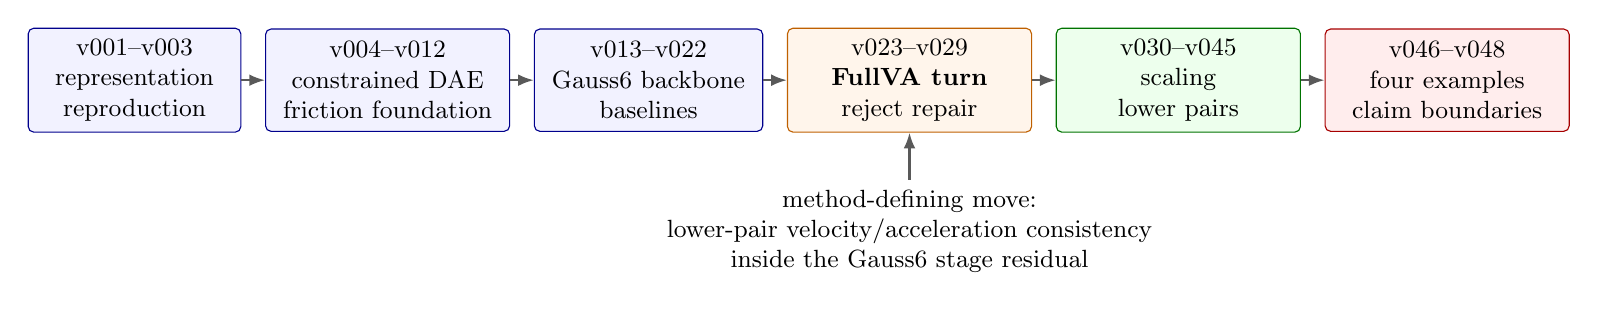
\begin{tikzpicture}[node distance=3.0mm and 3.0mm]
\node[box, minimum width=27mm, minimum height=13mm] (r) {v001--v003\\
representation\\reproduction};
\node[box, right=of r, minimum width=31mm, minimum height=13mm] (d) {v004--v012\\
constrained DAE\\friction foundation};
\node[box, right=of d, minimum width=29mm, minimum height=13mm] (g) {v013--v022\\
Gauss6 backbone\\baselines};
\node[warn, right=of g, minimum width=31mm, minimum height=13mm] (f) {v023--v029\\
\textbf{FullVA turn}\\reject repair};
\node[vbox, right=of f, minimum width=31mm, minimum height=13mm] (s) {v030--v045\\
scaling\\lower pairs};
\node[stop, right=of s, minimum width=31mm, minimum height=13mm] (b) {v046--v048\\
four examples\\claim boundaries};

\draw[arr] (r) -- (d);
\draw[arr] (d) -- (g);
\draw[arr] (g) -- (f);
\draw[arr] (f) -- (s);
\draw[arr] (s) -- (b);

\node[below=6mm of f, align=center, font=\small] (hinge) {method-defining
move:\\ lower-pair velocity/acceleration consistency\\ inside the Gauss6 stage
residual};
\draw[arr] (hinge.north) -- (f.south);
\end{tikzpicture}}
\caption{The 48-version discovery spine. Early versions make the state and
baseline interpretable, the middle versions keep Gauss6 while rejecting
endpoint-node and projection explanations, v026--v029 define the FullVA turn,
and later versions separate method evidence from scaling and external-claim
boundaries.}
\label{fig:discovery-spine}
\end{figure}

\begin{table}[!htbp]
\centering
\caption{Role-coded map of what the 48 versions contributed to the ledger.}
\label{tab:evolution}
\small
\begin{tabularx}{\linewidth}{p{0.06\linewidth}p{0.14\linewidth}p{0.31\linewidth}Y}
\toprule
\textbf{Role} & \textbf{Versions} & \textbf{Question and action} & \textbf{What survived for the final method} \\
\midrule
A & v001--v003 & Can SO(3) measurement, right-action kinematics, and a public
rA-style baseline be trusted? & Measurement and reproducibility became
prerequisites, not the new method. \\
B & v004--v005 & Can clean smooth Lie mechanics be high order without lower-pair
constraints? & High-order Lie/Gauss mechanics were feasible; the later problem
was constraint identity, not order in isolation. \\
C & v006--v012 & Which constraint levels, endpoint policies, friction regimes, AD
Jacobians, and $S^3$ transport choices change the one-step map? & ``The
integrator'' became a residual-identity and problem-specification object rather
than a formula name. \\
D & v013--v018 & Is Gauss6, adaptivity, trapezoidal/BDF, or Lobatto enough to
explain the high-order behavior? & Gauss6 stayed as the smooth backbone; reduced
baselines, adaptivity, and endpoint-node directions stayed verifier questions. \\
E & v019--v025 & Does multiplier-dependent friction plus a full revolute DAE make
endpoint-node or projection repairs sufficient? & Brown--McPhee-style loads were
representable, but direct Lobatto swaps and projection were rejected as method
identity. \\
F & v026--v029 & What residual object is missing in the full lower-pair DAE? &
Stage-level velocity and acceleration consistency entered the Gauss6 residual
and generalized from one pivot to an interbody FullVA path. \\
G & v030--v038 & Once FullVA enlarges Newton systems, can sparse/block
engineering be promoted as part of the method claim? & Sparse structure was
real, but backend correctness and wall-clock speed remained separate from
method validity. \\
H & v039--v045 & Does the FullVA/sparse route extend beyond a planar
double-revolute example? & Larger, skew-axis, prismatic, and row-colored
diagnostics broadened lower-pair coverage while keeping sparse speed open. \\
I & v046--v048 & What can the four ASME examples and external harness certify? &
Single/double carry accepted dynamic-order evidence; four-link/slider-crank
carry coverage; external superiority remains unpromoted. \\
\bottomrule
\end{tabularx}
\end{table}

\paragraph{A representative failure-to-constraint trace.}
The v023--v029 block shows the discovery mechanism in miniature. v023 moved the
search into the full absolute-coordinate revolute DAE and exposed endpoint
velocity defects. v024 rejected direct Lobatto endpoint-node replacement, and
v025 demoted projection because it repaired a symptom while changing the
trajectory map. The next constraint was therefore to move the missing
kinematic levels inside the stage solve: v026 inserted velocity rows, v027
inserted acceleration rows, v028 extended the idea toward off-axis lower-pair
constraints, and v029 showed that PivotVA/FullVA survived an interbody
double-revolute DAE. The 48-version history is scientifically useful for this
reason: it removes nearby explanations under verifier control, leaving
stage-level FullVA velocity/acceleration consistency as the method-defining
turn while later sparse, lower-pair, four-example, and external-comparison
versions manage boundaries rather than create a different claim.

\FloatBarrier

\section{Discovery Environment: Verifiers and Sandboxes}

The discovery environment represents a research state as
\[
  \mathcal{S}=(\mathcal{M},\mathcal{P},\mathcal{E},\mathcal{C},\mathcal{L}),
\]
where $\mathcal{M}$ is the method specification, $\mathcal{P}$ is the
benchmark specification, $\mathcal{E}$ is the evidence set, $\mathcal{C}$ is
the claim set, and $\mathcal{L}$ is the ledger containing version, proof,
validation, and package status. The agent may edit code and generate
experiments, but any transition in $\mathcal{C}$ is mediated by a verifier.
This is the environment in which the method was found: each candidate
integrator is allowed to run, but only the evidence that survives the relevant
validator can change the scientific state.
The verifier does not replace proof or numerical analysis; it controls claim
promotion so that diagnostics, coverage rows, and external harnesses cannot
silently become method, order, or superiority claims.

Operationally, a claim is promoted only if four checks pass: the named
one-step map has the same stage variables, residual rows, endpoint policy, and
solver tolerance; the mechanism, friction law, time window, step sizes, and
reference policy match the problem claim; the CSV/JSON/report/plot or proof
artifact exists; and the wording does not turn diagnostics into a larger claim,
such as mechanism coverage into dynamic order or an external harness into
superiority. A failed check leaves the result as hypothesis, diagnostic, open,
or forbidden instead of accepted.

The environment was initialized around three locks: an identity lock for stage
variables, row families, endpoint equations, tolerances, and backend policy; an
evidence lock binding each example to its problem, reference policy, step-size
set, artifact bundle, and gate role (order, interbody transfer, loop closure, or
mixed lower-pair coverage); and a claim lock recording which words are allowed
after evidence is produced. A failed run is useful because the verifier can say
which lock failed and can turn that failure into the next constraint.

\begin{table}[!htbp]
\centering
\caption{Durable objects maintained during method discovery.}
\label{tab:objects}
\small
\begin{tabularx}{\linewidth}{p{0.16\linewidth}YY}
\toprule
\textbf{Object} & \textbf{Contents} & \textbf{Purpose} \\
\midrule
MethodSpec & State space, stage variables, residual rows, endpoint policy,
solver tolerance, Jacobian backend & Prevents method drift while preserving a
stable method name. \\
ProblemSpec & Mechanism, parameters, drivers, friction law, time window, step
sizes, reference policy, metrics & Makes examples comparable across versions
and baselines. \\
EvidenceSpec & CSV rows, JSON summaries, plots, proof certificates, validator
outputs, PDFs & Defines what evidence can close a gate. \\
ClaimSpec & Claim text, status, required validators, nonpromotion rules,
forbidden wording & Stops diagnostic artifacts from becoming method claims. \\
Ledger & Version history, proof status, validation audits, package checks,
and claim-boundary files & Preserves both successful and rejected moves so the
discovery path can be reconstructed. \\
\bottomrule
\end{tabularx}
\end{table}

The working loop is to read ledgers, select an open gate, propose a bounded
hypothesis, choose a sandbox, run a verifier, and update evidence or claims.
This differs from a code-centric agent loop: the primary output is not a patch
but a controlled transition in scientific state, such as ``diagnostic only'',
``accepted method evidence'', or ``forbidden external-superiority claim''.
The loop is constructive because every failed promotion creates a narrower
next-version constraint rather than a discarded log. Table
\ref{tab:verdict-to-constraint} gives the recurring translation rule used in
the 48-version path.

\begin{table}[!htbp]
\centering
\caption{How verifier verdicts became next-version constraints.}
\label{tab:verdict-to-constraint}
\small
\begin{tabularx}{\linewidth}{p{0.23\linewidth}p{0.31\linewidth}Y}
\toprule
\textbf{Verifier verdict} & \textbf{Next constraint imposed on search} &
\textbf{Example from the path} \\
\midrule
Method identity mismatch & Split the diagnostic from the MethodSpec and test
the missing residual object directly. & Projection was demoted in v025; v026--v027
moved velocity and acceleration rows inside the stage solve. \\
Problem or reference drift & Freeze the ProblemSpec before comparing errors or
orders. & The double-pendulum claim used a method-side FullVA self-reference;
the v046 comparison stayed diagnostic. \\
Artifact/proof incomplete & Keep the claim open and move the result to a proof
or diagnostic lane. & Smooth slopes support sixth order, not a seventh-order
theorem; full \tfe{} replacement remains open. \\
Coverage without order theorem & Accept mechanism coverage while blocking
dynamic-order promotion. & Four-link and slider-crank close lower-pair reaction
channels but are not accepted asymptotic order rows. \\
Performance or source-policy caveat & Separate method validity from scaling and
external-superiority claims. & Sparse structure is retained without a speed
claim; v048 organizes same-test rows without superiority. \\
\bottomrule
\end{tabularx}
\end{table}

\paragraph{Sandbox levels.}
The verifier sandbox has four levels. L0 read-only validators ask whether
current claims match current artifacts. L1 bounded probes test one local
hypothesis without changing ledgers. L2 full generators regenerate method
artifacts after implementation changes. L3 source-policy campaigns compare to
external public-code baselines and require explicit authorization. A pass at
one level does not imply a pass at another. For example, a read-only artifact
validator can pass while an external-superiority or source-policy claim remains
false.

\paragraph{Claim states.}
Each claim is one of five states: hypothesis, diagnostic, accepted, open, or
forbidden. The important feature is reversibility. If a later verifier detects
reference-policy drift, stale prose, or a hidden proof assumption, the claim is
demoted rather than rationalized.

\section{Discovered Integrator Outcome: From Endpoint Repair to FullVA}

The anonymized case study covers a versioned research tree for lower-pair
Lie-group multibody integrator development. The project evolved from simple
$SO(3)$ kinematic checks to constrained DAE residuals, friction regimes,
sparse-Jacobian experiments, ASME mechanisms, proof audits, claim ledgers, and
source-policy external benchmark scaffolds. These files are not treated as
disposable logs; they are durable evidence objects that bind residual identity,
example role, proof status, and claim state.

The method discovery was not simply ``try Gauss6''. Gauss6 was the high-order
collocation backbone, but the accepted method emerged only after the pipeline
separated endpoint repair from residual identity. Direct endpoint-node and
Lobatto-style swaps were useful negative evidence. Projection closed visible
constraints but changed the trajectory map: it repaired an endpoint symptom,
whereas FullVA changed the residual being solved. The decisive turn was to
enforce velocity and acceleration consistency inside the stage residual, first
for a pivot joint and then as FullVA lower-pair rows. Table \ref{tab:pivots}
zooms in on the v023--v029 hinge where that method identity was separated from
endpoint repair.

\begin{table}[!htbp]
\centering
\caption{The FullVA hinge: why endpoint repair became stage-level velocity and
acceleration residuals.}
\label{tab:pivots}
\small
\begin{tabularx}{\linewidth}{p{0.13\linewidth}p{0.28\linewidth}YY}
\toprule
\textbf{Versions} & \textbf{Candidate explanation} & \textbf{Verifier outcome} & \textbf{Discovery consequence} \\
\midrule
v023 & A full absolute-coordinate revolute DAE is enough. &
Endpoint velocity defects and formulation fragility persisted. &
The missing object had to be inside the residual, not only in the
coordinate representation. \\
v024 & Replacing the endpoint node with a Lobatto/\tfe{}-style node will
recover the target behavior. & Direct full-DAE node replacement was
rank-deficient or divergent. & Node choice alone was rejected as the
method-defining change. \\
v025 & Projection can serve as the method identity because it closes visible
endpoint drift. & Projection repaired constraints but changed the trajectory
map. & Repair was demoted to a diagnostic, not accepted as the new
integrator. \\
v026--v027 & Add velocity, then acceleration, consistency rows inside the
Gauss6 stage solve. & The previously hidden velocity and acceleration channels
closed at the Newton residual level. & The method-defining object became
stage-level V/A consistency, not post-step correction. \\
v028--v029 & Test whether the pivot result is a single-joint artifact. &
Off-axis and interbody double-revolute checks preserved the same residual
logic. & FullVA became a lower-pair \method{} path rather than a
single-pendulum trick. \\
\bottomrule
\end{tabularx}
\end{table}

The hinge is therefore a three-gate filter rather than a label attached after a
successful run. After v025, reducing endpoint drift was no longer sufficient:
an acceptable candidate had to live inside the same Gauss6 stage solve, add the
missing lower-pair V/A rows to the MethodSpec itself, and survive off-axis or
interbody checks without changing the reference policy. v026--v029 are the
sequence that passed those gates. FullVA is the residual object left after
endpoint-node, projection, and single-joint explanations were rejected.

\subsection{Accepted method evidence}

The current accepted local method is \method{}, a three-stage Gauss-collocation
FullVA path. The accepted method claim is conditional sixth order. Smooth
projected position/velocity orders are 7.161/7.066, but the theorem-level
claim remains sixth order because retained proof conditions and solver
interfaces bound what can be stated. The residual implementation has a 132-row
boundary; the proof lane records a 96-row non-dynamic certificate and a
36-row Newton--Euler direct-substitution certificate for the current route.

The important method distinction is that FullVA is neither an output projection
nor a generic small-residual solve. In the accepted path, the MethodSpec itself
contains stage position, velocity, and acceleration consistency rows. This was
discovered because the pipeline kept projection repairs, endpoint-node
substitutions, and row-family substitutions as separate candidates. Several
candidates solved nonlinear systems with small residuals, but the verifier kept
them diagnostic when their rows, trajectory map, h-sweeps, or conditioning did
not match that MethodSpec. The discovery was therefore a narrowing process:
keep the Gauss6 smooth-order backbone, reject simple endpoint-node replacement,
reject projection as the method identity, and promote the FullVA residual
structure.

\subsection{Numerical test environment}

The four ASME mechanisms are not interchangeable demos. They form a verifier
ladder (Table \ref{tab:examples}): exact driven dynamics, interbody lower-pair
dynamics, closed-loop graph closure, and mixed closed-loop mechanism coverage.
Each rung carries its own ProblemSpec, EvidenceSpec, and ClaimSpec, so adding a
more complex mechanism does not automatically widen the theorem. At each rung
the validator asks a different question about method identity, selected by the
ambiguity the example can expose: clean order, interbody transfer, loop
closure, or mixed lower-pair coverage. The agent keeps the evidence types
distinct. Single and double pendulum are accepted local dynamic-order evidence.
Four-link and slider-crank are accepted mechanism coverage and closed-loop
consistency evidence, with maximum
closed-loop dynamic residuals of $1.338\times10^{-13}$ and
$6.492\times10^{-15}$, respectively, but they are not promoted to asymptotic
dynamic-order proof because the residual-to-error theorem remains open.

\begin{table}[!htbp]
\centering
\caption{Four-example verifier ladder and current claim boundary.}
\label{tab:examples}
\small
\begin{tabularx}{\linewidth}{p{0.18\linewidth}p{0.22\linewidth}YY}
\toprule
\textbf{Example} & \textbf{Verifier question} & \textbf{Accepted evidence} & \textbf{Boundary} \\
\midrule
Single pendulum & Can exact driven kinematics and an absolute-coordinate
FullVA residual carry a clean dynamic-order row? & Exact driven ASME
kinematics and absolute-coordinate driven FullVA residual; minimum accepted
order 6.024. & Supports local dynamic order, not external superiority. \\
Double pendulum & Does FullVA survive an interbody double-revolute joint under
a method-side self-reference policy? & Interbody double-revolute FullVA
self-reference; minimum accepted order 6.089. & Supports local dynamic order
under the accepted reference policy. \\
Four-link & Does a closed-loop lower-pair graph close kinematic, orientation,
and reaction-dynamics residual channels? & Closed-loop kinematic FullVA plus
reaction dynamics; max dynamics residual $1.338\times10^{-13}$. & Not promoted
to accepted asymptotic dynamic order. \\
Slider-crank & Does a mixed crank/slider closed loop close lower-pair
constraints and reaction residuals under the same policy? & Closed-loop
kinematic FullVA plus reaction dynamics; max dynamics residual
$6.492\times10^{-15}$. & Not promoted to accepted asymptotic dynamic order. \\
\bottomrule
\end{tabularx}
\end{table}

The ladder deliberately separates mechanism coverage from dynamic order. The
single-pendulum row uses an exact driven ASME trajectory and an
absolute-coordinate driven FullVA residual; over $h=\{0.2,0.1,0.05\}$ it
records position/velocity/orientation/angular-velocity orders
6.073/6.033/6.055/6.024. The double-pendulum row uses a double-revolute
FullVA local self-reference and records a minimum accepted order of 6.089. The
four-link and slider-crank rows use closed-loop kinematic FullVA plus reaction
dynamics on their lower-pair constraint graphs; they verify constraint,
orientation, and Newton--Euler reaction residual channels, but they are kept
as mechanism-coverage rows until either true dynamic trajectory/order rows or
a residual-to-error theorem closes the gap. This prevents a majority-vote
interpretation of the examples: four mechanisms in the evidence system does
not mean four dynamic-order proofs.

\begin{table}[!htbp]
\centering
\caption{Claim-state snapshot from the anonymized case-study artifacts.}
\label{tab:snapshot}
\small
\begin{tabularx}{\linewidth}{p{0.25\linewidth}p{0.23\linewidth}Y}
\toprule
\textbf{Artifact or claim} & \textbf{Current state} & \textbf{Why the state matters} \\
\midrule
\method{} method order & Accepted conditional sixth-order local method claim & Supported by smooth orders 7.161/7.066, residual-row certificates, and proof gates. \\
Four ASME examples & Accepted as mechanism coverage & Dynamic-order support is accepted for single and double pendulum only. \\
Four-link and slider-crank dynamic order & Open / nonpromoted & Residual checks are strong, but residual-to-error obligations remain open. \\
Full source-paper \tfe{} replacement & Open & Many formula and substitution diagnostics exist, but \status{full\_tfe\_stage\_replacement=false}. \\
Sparse runtime superiority & Open & Sparse structure is quantified, but dense automatic differentiation remains faster in measured wall time. \\
External source-policy superiority & Forbidden by current gate & The 44-row result matrix spans 11 methods and 4 examples, but source-policy rows remain open at 0/40. \\
\bottomrule
\end{tabularx}
\end{table}

\section{What the Failed Attempts Revealed}

The failed attempts became reusable verifier rules rather than a separate
failure narrative. Many \tfe{} substitutions, lower-pair closures, sparse
backends, and external-harness rows produced useful diagnostics, but remained
order-limited, rank-deficient, conditioning-limited, terminal-closure limited,
too slow, or source-policy open. The pipeline kept those rows because they
identified the ambiguity that had to be controlled before a method claim could
move from hypothesis or diagnostic to accepted.

\paragraph{Identity before score.}
Small changes to residual rows, endpoint variables, or solver policy can define
a different one-step map. The accepted method is therefore named by its
residual identity, \method{}, rather than by a broad family label such as
``Gauss'' or ``TFE''. A good local residual or a clean plot is not enough unless
the MethodSpec being solved is the one being claimed.

\paragraph{Repair before mechanism.}
Projection and endpoint-node repairs were useful because they showed what the
method could not be. A repair that closes a visible constraint after the step
does not have the same scientific meaning as putting the missing
velocity/acceleration rows inside the stage solve. This is the rule that turned
v026--v029 from a bug-fix sequence into the FullVA discovery.

\paragraph{Evidence type before promotion.}
The pipeline treats proof conditions, numerical slopes, mechanism coverage, and
external comparisons as different evidence types. Smooth finite-window slopes
support the conditional sixth-order claim, not a seventh-order theorem. Likewise
a closed-loop mechanism row can show that a complex example was mapped and its
reaction channels closed without proving asymptotic dynamic order.

\paragraph{Policy before comparison.}
External baselines require matched time windows, reference states, error norms,
work metrics, and source-policy rows. The same-test harness organizes future
comparison work, but the claim ledger prevents local diagnostics from becoming
public-code superiority claims.

\section{Discussion, Limitations, and Conclusion}

The case study suggests a specific role for LLM agents in method discovery:
not replacing mathematical or engineering judgment, but keeping code, residual
identity, example role, proof status, reference policy, and nonpromotion memory
together long enough for technical lessons to accumulate. The main result is
therefore a verifier-centered discovery method for finding integrators, with
\method{} as the discovered outcome rather than the whole subject of the paper.
In the 48-version run, endpoint repair and reduced surrogates gave way to
stage-level FullVA residuals inside the nonlinear solve, yielding the
conditional sixth-order \method{} result.

The evidence is a single anonymized scientific-computing case study, not a
multi-lab benchmark, and the current paper does not release a fully anonymized
artifact bundle. The method claim remains deliberately bounded: conditional
sixth-order \method{}, not complete source-paper \tfe{} reproduction, sparse
runtime superiority, or external superiority. Useful research agents should be
evaluated by whether they can discover methods while preserving the auditable
path, rejected alternatives, and nonpromotion boundaries around those methods.

\paragraph{AI assistance disclosure.}
This manuscript draft was prepared with assistance from an AI coding assistant
that inspected the local artifact tree, checked the LM4Sci 2026 call for
papers, and drafted the anonymized LaTeX source. The authors are responsible
for verifying all claims, citations, artifact boundaries, and final submission
compliance.

\bibliographystyle{plainnat}
\bibliography{references}

\clearpage
\appendix

\section{Expanded 48-Version Discovery Ledger}

This appendix records the detailed discovery path behind Table
\ref{tab:evolution}. The entries are intentionally concise: each version is
included because it changed the hypothesis space for the next version. The
ledger should be read as a sequence of method-discovery constraints, not as a
list of independent experiments. The recurring question is what each version
calibrated, rejected, promoted, or quarantined. Each entry can be expanded into
the same tuple: candidate explanation, bounded artifact, verifier verdict, next
constraint, and claim-state movement. A failed version can therefore carry
positive scientific information when it rules out a nearby method identity,
fixes a reference policy, or prevents a diagnostic from becoming a stronger
claim.

\subsection{Representation, Reproduction, and Conservative Mechanics}

\paragraph{v001.}
The pipeline began with reproducible $SO(3)$ benchmarks for prescribed
rotations and torque-free rigid-body dynamics. This did not discover a method,
but it created stable error and invariant measurements that later versions
could reuse.

\paragraph{v002.}
The right-action CF4/RKMK4 kinematic formulas were corrected and verified at
fourth order. This established that the representation and local Lie update
conventions could be made reliable before adding constraints.

\paragraph{v003.}
The SBEL/Negrut rA path was reproduced as a local reference anchor. The tested
behavior was not a high-order competitor, but the version fixed a reproducible
baseline for later ASME-style examples.

\paragraph{v004.}
A Yoshida-composed Lie midpoint method gave fourth-order conservative
mechanics with good invariants. Its negative substeps made it a poor candidate
for friction/contact, which pushed the search toward Gauss collocation.

\paragraph{v005.}
Two-stage Gauss-Legendre Lie4 improved smooth conservative mechanics without
negative substeps. The limitation was that it still had no constrained DAE
structure.

\subsection{From Reduced DAE to Quaternion Endpoint DAE}

\paragraph{v006.}
Gauss-Lie4 was moved to a reduced fixed-pivot DAE with recovered reactions.
This showed that high order and constraints could coexist, but only in a
reduced formulation rather than a full absolute-coordinate Newton solve.

\paragraph{v007.}
The first absolute-coordinate stage DAE introduced explicit multipliers and
showed that position, velocity, and acceleration consistency are all relevant
for index-3 behavior. Endpoint projection was still outside Newton.

\paragraph{v008.}
Endpoint variables and endpoint constraints were placed inside the nonlinear
solve. This removed post-step endpoint projection in the fixed-pivot setting
and exposed the need for a faster Jacobian backend.

\paragraph{v009.}
Regularized friction was added to the endpoint DAE. Smooth friction preserved
high order, while sharper friction produced order reduction; this made
friction smoothness a first-class experimental variable.

\paragraph{v010.}
JAX automatic differentiation replaced finite-difference Jacobians. The
solution matched finite differences while greatly improving local solve speed,
but the residual still used an $SO(3)$ local-vector representation.

\paragraph{v011.}
The quaternion transport operators were checked independently. This made the
source-style $S^3$ derivative map a verified component, but it was not yet an
integrator residual.

\paragraph{v012.}
The endpoint DAE was rebuilt with scalar-first unit quaternions. It matched the
previous $SO(3)$ residual behavior while preserving unit norm, but it was still
fourth order and sharp-friction limited.

\subsection{High-Order Candidate, Friction, and Local Baselines}

\paragraph{v013.}
Three-stage Gauss6 endpoint collocation was added. Smooth friction reached
near-sixth-order behavior, establishing Gauss6 as the main high-order
backbone.

\paragraph{v014.}
A friction smoothness sweep identified where Gauss6 was a strong win and where
near-nonsmooth behavior became marginal. This turned friction regularization
into an explicit decision boundary.

\paragraph{v015.}
An embedded adaptive Gauss6/Gauss4 controller improved high-accuracy runs in
near-sharp regimes. It helped with difficult friction windows but was not the
fixed-step method identity.

\paragraph{v016.}
A favorable reduced Lie-trapezoidal baseline was added. Gauss6 dominated it in
local accuracy, so the trapezoidal direction became a baseline rather than the
main discovery route.

\paragraph{v017.}
A reduced Lie-BDF2 baseline was added. It was useful as a damping/robustness
reference, but not as the high-accuracy winner.

\paragraph{v018.}
A reduced Lie-Lobatto endpoint-node baseline tested the TFE-like nodal
direction. It was accurate but slower, suggesting that endpoint nodes alone
were not enough.

\paragraph{v019.}
Multiplier-dependent Stribeck-style friction was inserted into the residual.
This showed that AD could handle friction laws coupled to reaction loads.

\paragraph{v020.}
Adaptive control was combined with multiplier-dependent friction. It improved
sharp lambda-friction accuracy, but it remained a smooth regularized model.

\paragraph{v021.}
Brown--McPhee-style continuous friction replaced the simpler lambda-friction
law. The route was promising for sharp friction but still a fixed-pivot
surrogate.

\paragraph{v022.}
A one-degree-of-freedom revolute Brown--McPhee benchmark moved the example
closer to the target mechanism class. It remained reduced and therefore could not close the full
absolute-coordinate lower-pair claim.

\subsection{The FullVA Turn}

\paragraph{v023.}
A five-constraint absolute-coordinate revolute DAE was introduced. It exposed
endpoint velocity defects and showed that robustness in a full DAE required
more than the reduced Gauss6 construction.

\paragraph{v024.}
Direct Lobatto endpoint-node collocation was tested in the full revolute DAE.
The failure was decisive: a simple Gauss-to-Lobatto node swap was
rank-deficient or divergent, so the missing method was not just a nodal swap.

\paragraph{v025.}
SHAKE/RATTLE-style endpoint projection repaired visible endpoint drift and
rescued some sharp cases. The cost was that projection changed trajectory
accuracy, so it could not become the method identity.

\paragraph{v026.}
Stage pivot-velocity constraints were moved inside the square residual. This
reduced endpoint velocity drift without relying on projection and pointed to
in-residual velocity consistency.

\paragraph{v027.}
Stage pivot-acceleration constraints were added. Endpoint velocity drift
dropped to roundoff-scale values, making velocity-plus-acceleration residuals
the leading repair idea.

\paragraph{v028.}
Off-axis torque and hinge-axis velocity/acceleration rows were added. The
diagnostic confirmed that axis consistency could be enforced without changing
the one-joint trajectory bottleneck, so the next step had to be multi-joint
and lower-pair generalization.

\paragraph{v029.}
A two-body double-revolute DAE showed that PivotVA/FullVA generalized to an
interbody joint. It also exposed a 138D Newton system and made sparse/block
linear algebra unavoidable.

\subsection{Sparse Solver Search}

\paragraph{v030.}
The double-revolute Jacobian was measured as highly sparse. This justified
sparse Newton work but also showed that dense AD materialization was the next
cost bottleneck.

\paragraph{v031.}
CSR sparse linear solves were integrated into the Newton loop. They preserved
the trajectory and improved targeted solve time, but dense Jacobian
materialization remained.

\paragraph{v032.}
Matrix-free JVP plus unpreconditioned GMRES was tested. It failed as a default
solver path, showing that correctness of JVP products was not enough without
preconditioning or structure.

\paragraph{v033.}
Lagged sparse Newton reused CSR Jacobians. It preserved trajectories but did
not give a meaningful end-to-end speed win, ruling out simple Jacobian lagging.

\paragraph{v034.}
Column-colored JVP sparse assembly matched dense Jacobians but was slower in
the small 138D system. This separated sparse correctness from sparse speed.

\paragraph{v035.}
Batched colored JVPs improved the sparse-AD path and became the best
double-revolute structured sparse-AD backend, but still depended on a dense
warm-up pattern.

\paragraph{v036.}
A block-symbolic sparsity pattern avoided dense warm-up discovery. It was
correct but conservative and overcolored.

\paragraph{v037.}
JVP-pruned pattern discovery recovered the exact observed sparse pattern
without dense Jacobian materialization. It remained path-sampled rather than a
symbolic proof.

\paragraph{v038.}
Cached pattern reuse tested whether a discovered sparse pattern could survive
nearby smooth and sharp regimes. It worked locally and introduced a cache
policy.

\paragraph{v039.}
The sparse path was moved to a triple-revolute topology. This was the first
larger-topology scaling evidence.

\paragraph{v040.}
A generated block superset plus pruning replaced the earlier full-matrix
superset. This was a more production-like sparse pattern route.

\paragraph{v041.}
Cache refresh and union rules were added for triple-revolute runs. This made
sparse-pattern reuse safer without dense Jacobians.

\paragraph{v042.}
Skew-axis triple-revolute lower-pair geometry moved beyond planar chains. This
showed that FullVA and sparse diagnostics could handle non-coplanar geometry.

\paragraph{v043.}
A skew prismatic joint added the first non-revolute lower-pair coverage. Sparse
AD remained correctness-valid but was not faster at this size.

\paragraph{v044.}
An interbody double-prismatic system added another non-revolute lower-pair
case. The 90-color pattern made sparse AD slower, motivating row-color and
block-assembly diagnostics.

\paragraph{v045.}
Row-colored VJP reduced the sparse seed count for the prismatic case but did
not beat dense \texttt{jacfwd}. The sparse-solver line became a quantified
caveat rather than an accepted speed claim.

\subsection{Four-Example Validation and Cross-Paper Harness}

\paragraph{v046.}
The four ASME-style examples were introduced as a validation anchor:
single-pendulum, double-pendulum, four-link, and slider-crank. This was a
reproducibility and coverage harness, not a new \method{} claim.

\paragraph{v047.}
The cylindrical lower-pair scaffold became the current method discovery
version. It records the accepted \method{} path and smooth observed
position/velocity orders 7.161/7.066. It also records four-example method
evidence, many full-TFE replacement diagnostics, and explicit caveats around
sparse speed, source-paper TFE replacement, and sharp-friction coarse behavior.

\paragraph{v048.}
The cross-paper same-test benchmark harness was added for external comparison
work. It executes and organizes public-code and local comparison rows, but it
does not promote an external-superiority claim; source-policy rows remain open.

\section{Numerical Examples and Claim Roles}

The four numerical examples have different scientific roles. The
single-pendulum example supplies exact driven kinematics and an
absolute-coordinate driven FullVA residual. The double-pendulum example
supplies dynamic-order evidence through a double-revolute FullVA
self-reference policy. The four-link and slider-crank examples supply
closed-loop lower-pair mechanism coverage, constraint closure, and
reaction-dynamics residual checks. They do not by themselves close asymptotic
dynamic order because the residual-to-error theorem is still open.

The test policy also separates routine evidence from heavy external campaigns.
Routine method evidence uses bounded local h-sweeps and read-only validators.
Strict public-policy rows, source-policy execution, and apples-to-apples
external-superiority claims require separate gates. This is why the
method-discovery claim can be accepted while complete source-paper TFE
reproduction and external superiority remain unaccepted.

\end{document}
